
\section{System Architecture}

\subsection{Permuter Design}
The Nash cipher's core component is a permuter that implements two different state transition paths, labeled as ``red'' and ``blue''. Each path includes both state transitions and bit transformations.

\begin{figure}[H]
    \centering
    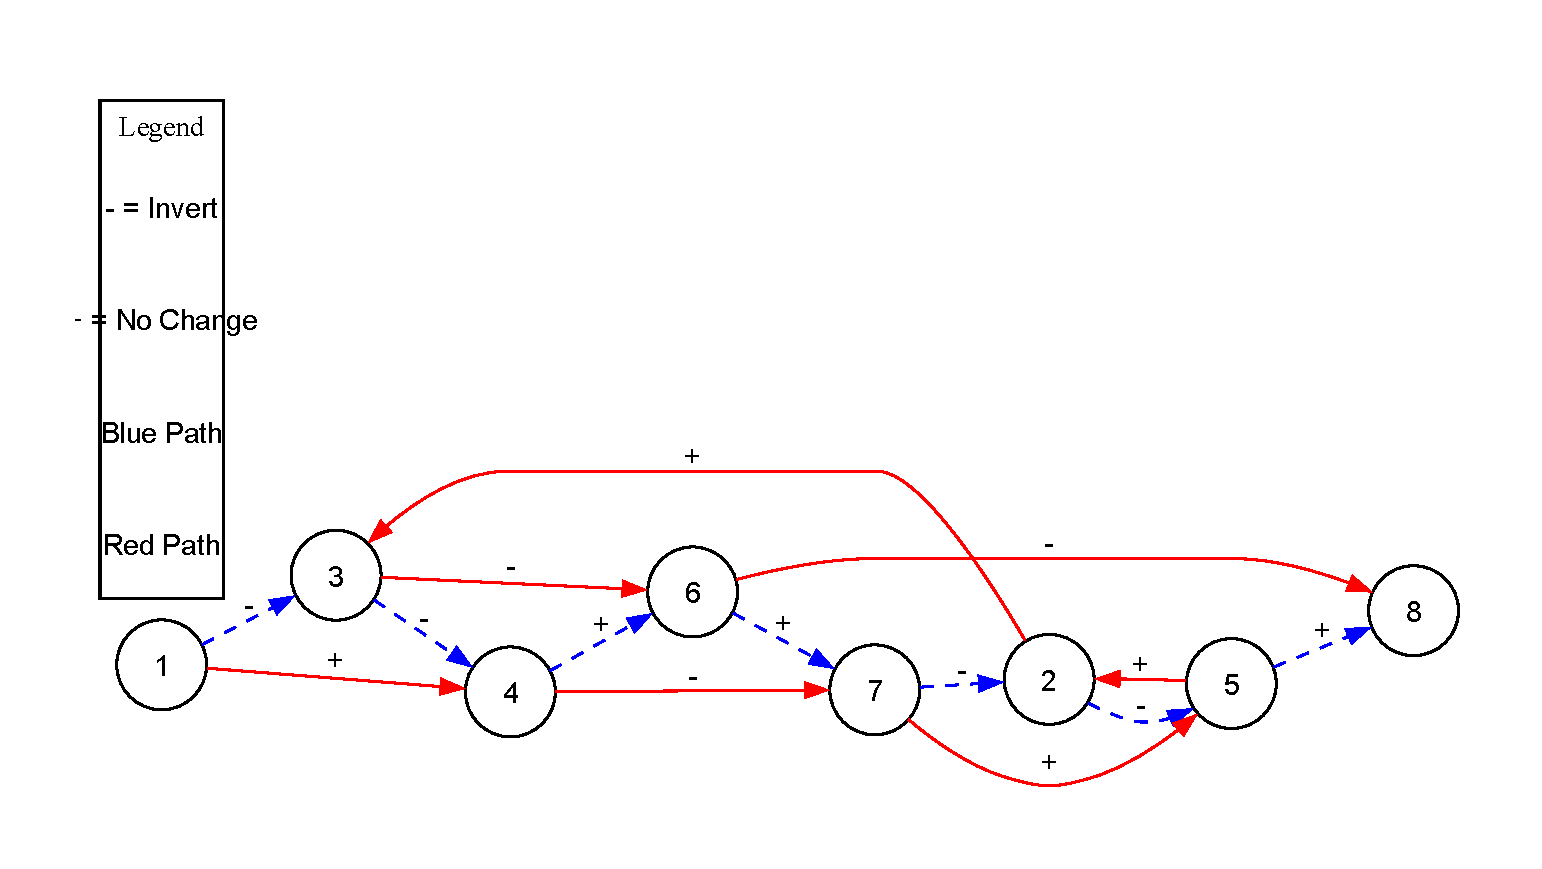
\includegraphics[width=0.8\textwidth]{figures/permuter.pdf}
    \caption{Nash Permuter State Machine. Red (solid) and blue (dashed) paths show different state transitions. The + and - labels indicate whether the bit is preserved or inverted during transition.}
    \label{fig:permuter}
\end{figure}

\subsection{Transmitting Arrangement}
The transmitting arrangement combines the permuter with a feedback mechanism through an adder (binary addition modulo 2) and a decider that selects between red and blue permutation paths.

\begin{figure}[H]
    \centering
    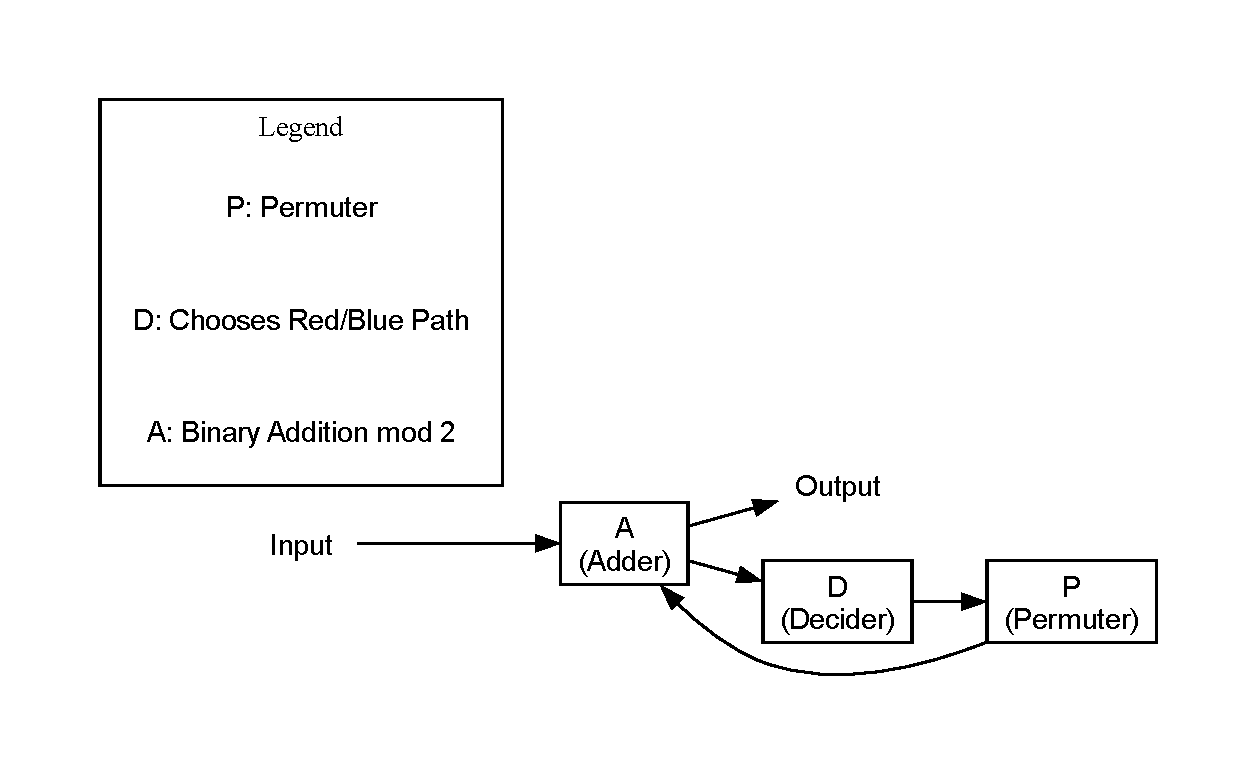
\includegraphics[width=0.8\textwidth]{figures/transmitter.pdf}
    \caption{Nash Cipher Transmitting Arrangement. The adder A performs binary addition modulo 2, decider D selects between red and blue permutation paths based on the adder output, and permuter P performs the state transitions and bit transformations.}
    \label{fig:transmitter}
\end{figure}

\subsection{Receiving Arrangement}
The receiving arrangement mirrors the transmitting arrangement but includes a retarder (one-unit delay) to synchronize the input with the permuter output.

\begin{figure}[H]
    \centering
    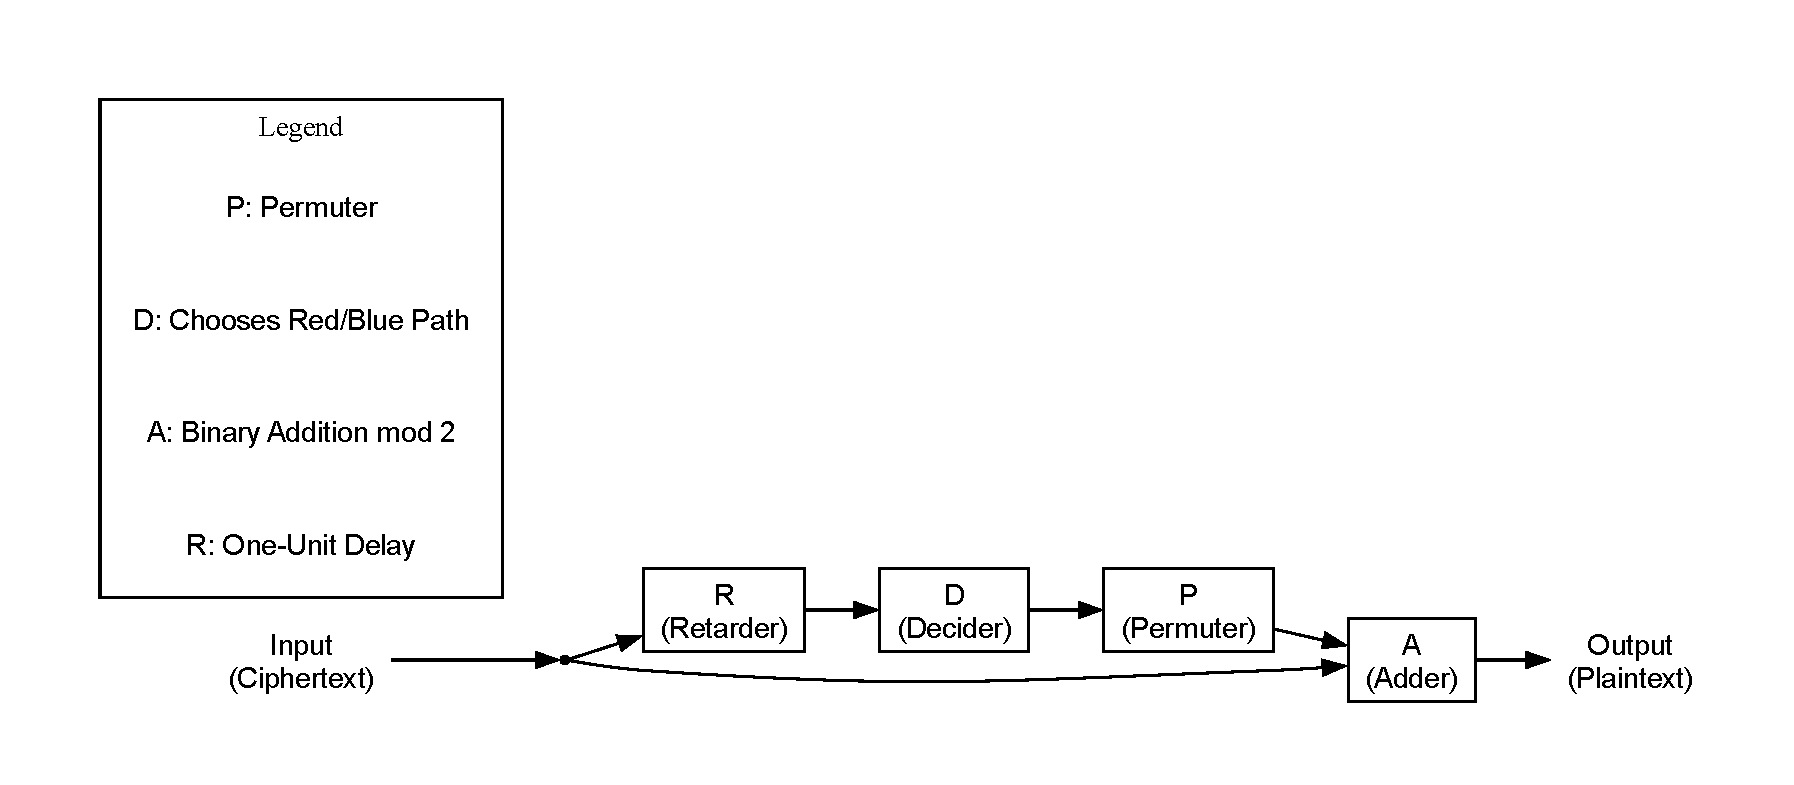
\includegraphics[width=0.8\textwidth]{figures/receiver.pdf}
    \caption{Nash Cipher Receiving Arrangement. The retarder R provides a one-unit delay to synchronize the input with the permuter output. The remaining components function identically to the transmitting arrangement.}
    \label{fig:receiver}
\end{figure}

\section{Key Structure}

The implementation accepts 128-bit keys formatted as hexadecimal values. The key space is structured as follows:

\begin{itemize}
    \item First 64 bits: Red permutation table
    \begin{itemize}
        \item Bits 0-31: Next state mappings
        \item Bits 32-63: Transform functions
    \end{itemize}
    \item Last 64 bits: Blue permutation table
    \begin{itemize}
        \item Bits 64-95: Next state mappings
        \item Bits 96-127: Transform functions
    \end{itemize}
\end{itemize}

\subsection{Key Validation}

Each key must satisfy the following requirements:
\begin{enumerate}
    \item All next state values must be valid (0-7)
    \item Transform functions must be binary (0 or 1)
    \item State transitions must form complete cycles
\end{enumerate}

\subsection{Example Key Format}
Keys are represented in hexadecimal format:
\begin{verbatim}
[<:AA9987E016931D993B2359B1103A88C6:>]
\end{verbatim}

This notation ensures consistent key handling across different implementations while maintaining compatibility with standard cryptographic interfaces.

\section{Implementation Considerations}

\subsection{State Machine Implementation}
The cipher's state machine requires...

[Note: Additional implementation details to be added]